\documentclass[conference]{IEEEtran}
\usepackage{cite}
\usepackage{amsmath}
\usepackage{graphicx}
\usepackage{booktabs}
\usepackage{url}
\graphicspath{{../docs/figures/}}
% generated by scripts/metrics_to_tex.py from results/metrics.json -- do not edit
\newcommand{\metric}[1]{\ifcsname metric@#1\endcsname\csname metric@#1\endcsname\else\errmessage{missing metric #1}\fi}

\expandafter\def\csname metric@cmp.csla4.adp\endcsname{294}
\expandafter\def\csname metric@cmp.csla4.area_um2\endcsname{236}
\expandafter\def\csname metric@cmp.csla4.cell_count\endcsname{15}
\expandafter\def\csname metric@cmp.csla4.delay_ns\endcsname{1.24}
\expandafter\def\csname metric@cmp.csla4.nand2_eq\endcsname{63}
\expandafter\def\csname metric@cmp.csla4_flat.adp\endcsname{180}
\expandafter\def\csname metric@cmp.csla4_flat.area_um2\endcsname{113}
\expandafter\def\csname metric@cmp.csla4_flat.cell_count\endcsname{18}
\expandafter\def\csname metric@cmp.csla4_flat.delay_ns\endcsname{1.59}
\expandafter\def\csname metric@cmp.csla4_flat.nand2_eq\endcsname{30}
\expandafter\def\csname metric@cmp.rca4.adp\endcsname{231}
\expandafter\def\csname metric@cmp.rca4.area_um2\endcsname{135}
\expandafter\def\csname metric@cmp.rca4.cell_count\endcsname{8}
\expandafter\def\csname metric@cmp.rca4.delay_ns\endcsname{1.71}
\expandafter\def\csname metric@cmp.rca4.nand2_eq\endcsname{36}
\expandafter\def\csname metric@cmp.rca4_flat.adp\endcsname{218}
\expandafter\def\csname metric@cmp.rca4_flat.area_um2\endcsname{109}
\expandafter\def\csname metric@cmp.rca4_flat.cell_count\endcsname{14}
\expandafter\def\csname metric@cmp.rca4_flat.delay_ns\endcsname{2}
\expandafter\def\csname metric@cmp.rca4_flat.nand2_eq\endcsname{29}
\expandafter\def\csname metric@env.magic_version\endcsname{8.3.685}
\expandafter\def\csname metric@env.ngspice_version\endcsname{ngspice-47 : Circuit level simulation program}
\expandafter\def\csname metric@env.openlane_version\endcsname{LibreLane v3.0.16}
\expandafter\def\csname metric@env.pdk_hash\endcsname{8afc8346a57fe1ab7934ba5a6056ea8b43078e71}
\expandafter\def\csname metric@env.verilator_version\endcsname{Verilator 5.052 2026-09-05 rev v5.052}
\expandafter\def\csname metric@env.yosys_version\endcsname{Yosys 0.66 (git sha1 86f2ddebc-dirty, g++ 16.1.1 -march=x86-64 -mtune=generic -O2 -fno-plt -fexceptions -fstack-clash-protection -fcf-protection -fno-omit-frame-pointer -mno-omit-leaf-frame-pointer -ffile-prefix-map=/build/yosys/src=/usr/src/debug/yosys -fPIC -O3) [startdir/yosys at makepkg]}
\expandafter\def\csname metric@fa.area_um2\endcsname{200}
\expandafter\def\csname metric@fa.drc_errors\endcsname{0}
\expandafter\def\csname metric@fa.height_um\endcsname{12.3}
\expandafter\def\csname metric@fa.lvs_match\endcsname{true}
\expandafter\def\csname metric@fa.ntrans\endcsname{28}
\expandafter\def\csname metric@fa.pex_cap_count\endcsname{80}
\expandafter\def\csname metric@fa.s1.delay_pre_ps\endcsname{306}
\expandafter\def\csname metric@fa.s2.delay_pre_ps\endcsname{264}
\expandafter\def\csname metric@fa.sizing_chosen\endcsname{S2}
\expandafter\def\csname metric@fa.taps\endcsname{2}
\expandafter\def\csname metric@fa.width_um\endcsname{16.2}
\expandafter\def\csname metric@le.B\endcsname{31.5}
\expandafter\def\csname metric@le.D_est_ps\endcsname{312}
\expandafter\def\csname metric@le.D_est_tau\endcsname{24.2}
\expandafter\def\csname metric@le.F\endcsname{183}
\expandafter\def\csname metric@le.G\endcsname{4}
\expandafter\def\csname metric@le.H\endcsname{1.45}
\expandafter\def\csname metric@le.N\endcsname{4}
\expandafter\def\csname metric@le.c_mux_s_ff\endcsname{3.4}
\expandafter\def\csname metric@le.err_post_pct\endcsname{-25.7}
\expandafter\def\csname metric@le.err_pre_pct\endcsname{18.2}
\expandafter\def\csname metric@le.fhat\endcsname{3.68}
\expandafter\def\csname metric@le.fo4_ps\endcsname{64.5}
\expandafter\def\csname metric@le.p_carry\endcsname{3.6}
\expandafter\def\csname metric@le.pinv\endcsname{1.13}
\expandafter\def\csname metric@le.tau_ps\endcsname{12.9}
\expandafter\def\csname metric@le.wn_unit_um\endcsname{0.42}
\expandafter\def\csname metric@le.wp_unit_um\endcsname{0.84}
\expandafter\def\csname metric@pnr.antenna_violations\endcsname{0}
\expandafter\def\csname metric@pnr.cell_count\endcsname{137}
\expandafter\def\csname metric@pnr.core_util_pct\endcsname{81}
\expandafter\def\csname metric@pnr.die_area_um2\endcsname{3420}
\expandafter\def\csname metric@pnr.drc_klayout\endcsname{0}
\expandafter\def\csname metric@pnr.drc_magic\endcsname{0}
\expandafter\def\csname metric@pnr.fmax_mhz\endcsname{277}
\expandafter\def\csname metric@pnr.lvs_errors\endcsname{0}
\expandafter\def\csname metric@pnr.power_total_mw\endcsname{0.342}
\expandafter\def\csname metric@pnr.wirelength_um\endcsname{2200}
\expandafter\def\csname metric@pnr.wns_hold_ns\endcsname{0.327}
\expandafter\def\csname metric@pnr.wns_hold_worst_corner_ns\endcsname{0.111}
\expandafter\def\csname metric@pnr.wns_setup_ns\endcsname{6.39}
\expandafter\def\csname metric@pnr.wns_setup_worst_corner_ns\endcsname{4.8}
\expandafter\def\csname metric@pnr5.status\endcsname{FAIL}
\expandafter\def\csname metric@pnr5.wns_hold_ns\endcsname{0.326}
\expandafter\def\csname metric@pnr5.wns_hold_worst_corner_ns\endcsname{0.11}
\expandafter\def\csname metric@pnr5.wns_setup_ns\endcsname{1.39}
\expandafter\def\csname metric@pnr5.wns_setup_worst_corner_ns\endcsname{-0.045}
\expandafter\def\csname metric@sim.case1.status\endcsname{PASS}
\expandafter\def\csname metric@sim.case2.status\endcsname{PASS}
\expandafter\def\csname metric@sim.case3.status\endcsname{PASS}
\expandafter\def\csname metric@sim.case4.status\endcsname{PASS}
\expandafter\def\csname metric@sim.case5.status\endcsname{PASS}
\expandafter\def\csname metric@sim.case_illegal.status\endcsname{PASS}
\expandafter\def\csname metric@sim.cycles_per_result\endcsname{2}
\expandafter\def\csname metric@sim.exhaustive.checked\endcsname{512}
\expandafter\def\csname metric@sim.exhaustive.errors\endcsname{0}
\expandafter\def\csname metric@sim.latency_cycles\endcsname{2}
\expandafter\def\csname metric@sim.unit_csla4.checked\endcsname{512}
\expandafter\def\csname metric@sim.unit_csla4.errors\endcsname{0}
\expandafter\def\csname metric@spice.D_post_ps\endcsname{420}
\expandafter\def\csname metric@spice.D_pre_ps\endcsname{264}
\expandafter\def\csname metric@sta.synth.crit_arrival_ns\endcsname{1.78}
\expandafter\def\csname metric@sta.synth.crit_path\endcsname{a\_q[0] -> cout\_q}
\expandafter\def\csname metric@sta.synth.wns_hold_ns\endcsname{0.243}
\expandafter\def\csname metric@sta.synth.wns_setup_ns\endcsname{6.78}
\expandafter\def\csname metric@sta.synth.worst_path\endcsname{valid\_in -> a\_q[0]}
\expandafter\def\csname metric@synth.nand2_area_um2\endcsname{3.75}
\expandafter\def\csname metric@synth.top.area_um2\endcsname{817}
\expandafter\def\csname metric@synth.top.cell_count\endcsname{49}
\expandafter\def\csname metric@synth.top.ff_count\endcsname{16}
\expandafter\def\csname metric@synth.top.latch_count\endcsname{0}
\expandafter\def\csname metric@synth.top.nand2_eq\endcsname{218}

\newcommand{\um}{\,$\mu$m}
\newcommand{\umsq}{\,$\mu$m$^2$}

\begin{document}

\title{CarrySelect-4: A Registered 4-bit Carry-Select Adder from RTL to GDSII in SKY130 with a Logical-Effort Study of a Full-Custom Mirror Full Adder}

\author{\IEEEauthorblockN{Nguy Quoc Trung (23CE.B026) and Nguyen Minh Anh Tu (23CE085)}
\IEEEauthorblockA{Group 7, CE2032 VLSI Design, Faculty of Computer Engineering and Electronics\\
Vietnam--Korea University of Information and Communication Technology (VKU), Da Nang, Vietnam\\
trungnq.23ceb@vku.udn.vn, tunma.23ce@vku.udn.vn}}

\maketitle

\begin{abstract}
We present CarrySelect-4, a 4-bit carry-select adder (CSLA) wrapped in a valid/ready interface and
taken through a complete open-source flow on the SkyWater SKY130 process. The datapath splits the
adder into a 2-bit ripple block and two speculative 2-bit blocks whose results are selected by the
low carry; a three-state Moore controller registers inputs and outputs, giving a latency of
\metric{sim.latency_cycles} cycles and one result every \metric{sim.cycles_per_result} cycles.
Exhaustive self-checking simulation passes \metric{sim.exhaustive.checked} of
\metric{sim.exhaustive.checked} input vectors. Synthesis with Yosys uses
\metric{synth.top.nand2_eq} NAND2 equivalents, and LibreLane places and routes the design at
100\,MHz with positive setup and hold slack in all nine signoff corners and zero DRC and LVS errors.
In a second branch we size, lay out and extract a 28-transistor mirror full adder in Magic and
compare a Logical Effort estimate of the ripple-carry path with pre- and post-layout SPICE: the
estimate of \metric{le.D_est_ps}\,ps lies between the schematic result
(\metric{spice.D_pre_ps}\,ps) and the extracted result (\metric{spice.D_post_ps}\,ps).
\end{abstract}

\begin{IEEEkeywords}
carry-select adder, SKY130, OpenLane, LibreLane, logical effort, full-custom layout, mirror adder
\end{IEEEkeywords}

\section{Introduction}
The carry chain sets the delay of an $n$-bit ripple-carry adder (RCA), which grows as $O(n)$.
A carry-select adder~\cite{bedrij1962} computes the upper bits twice, once for each value of the
incoming carry, and picks the right result with a multiplexer, trading area for delay~\cite{weste2010}.
This work implements a small but complete instance of that idea and follows it through every step
of a modern open-source flow: RTL and verification, synthesis and static timing with
Yosys~\cite{yosys} and OpenSTA~\cite{opensta}, and physical design with OpenLane~2 / LibreLane~\cite{openlane,librelane}
on SKY130~\cite{skywater}. We then study the adder's leaf cell, a mirror full adder, at transistor
level with Logical Effort~\cite{sutherland1999} and Magic~\cite{magic}, and check how well the hand
estimate predicts SPICE before and after layout.

\section{Architecture}
Fig.~\ref{fig:block} shows the top level. The 9-bit input word $\{c_{in}, b, a\}$ is captured in an
input bank (9 FF) when \texttt{ld\_en = valid\_in \& ready\_out}. The CSLA uses six full adders in
three 2-bit RCAs: \emph{low} adds $a[1{:}0]+b[1{:}0]+c_{in}$, while \emph{hi0} and \emph{hi1} add
$a[3{:}2]+b[3{:}2]$ with a carry-in of 0 and 1. The low carry $c_2$ drives the select inputs of three
2:1 multiplexers for \texttt{sum[3:2]} and \texttt{cout}. Full adder and multiplexer modules keep
their hierarchy during synthesis so that the carry-select structure survives technology mapping.
The 5-bit result is stored in an output bank (5 FF). A Moore controller with two state bits
(Fig.~\ref{fig:fsm}) sequences IDLE, COMPUTE and DONE; the unused code returns to IDLE. All
\metric{synth.top.ff_count} flip-flops use an asynchronous active-low reset.

\begin{figure}[t]
\centering
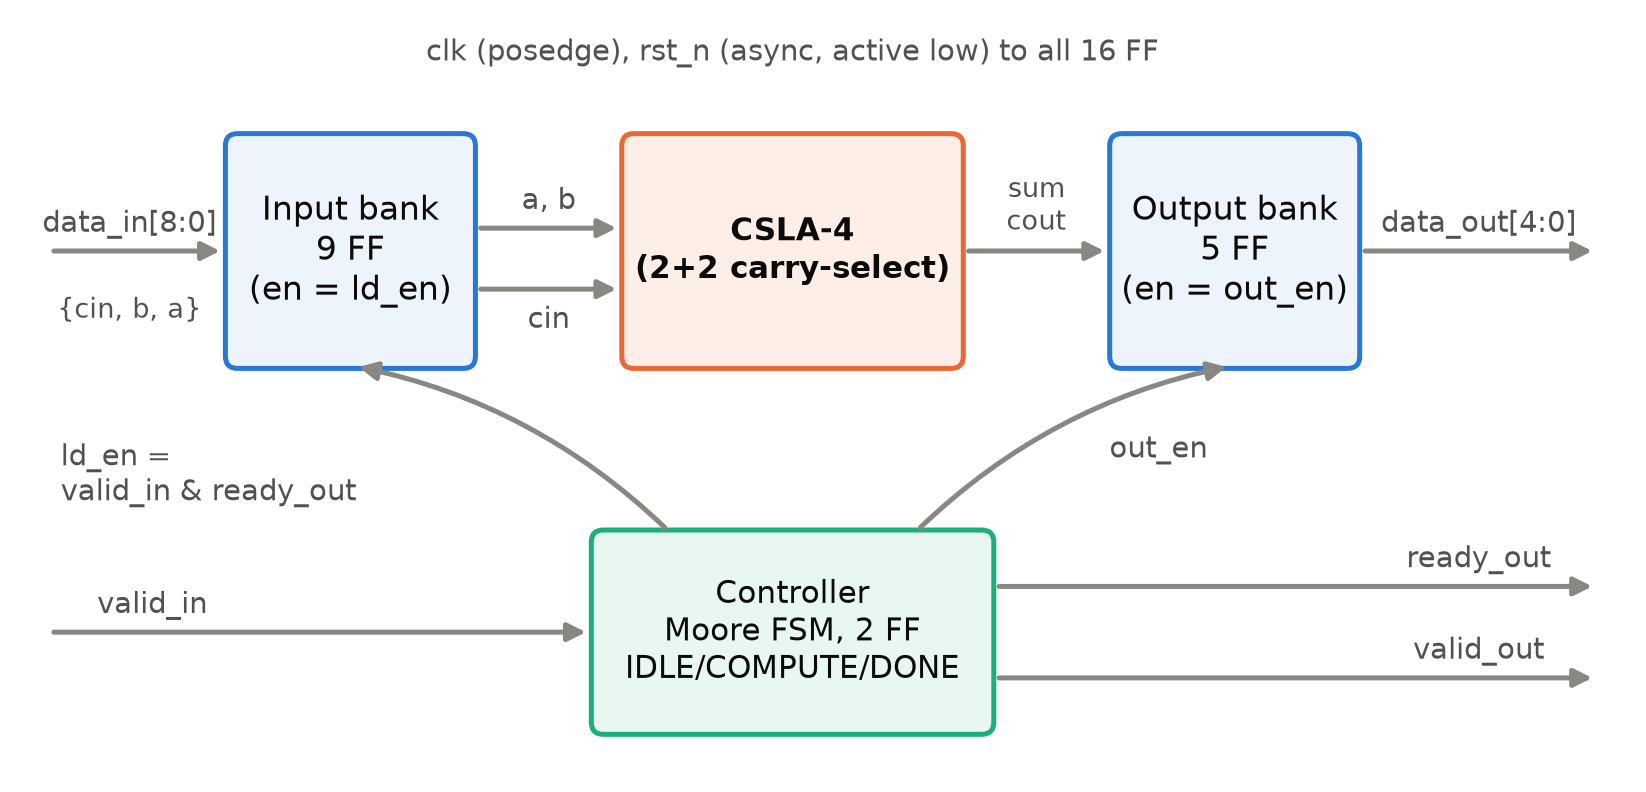
\includegraphics[width=\columnwidth]{block_diagram.png}
\caption{Registered CarrySelect-4 datapath and controller.}
\label{fig:block}
\end{figure}

\begin{figure}[t]
\centering
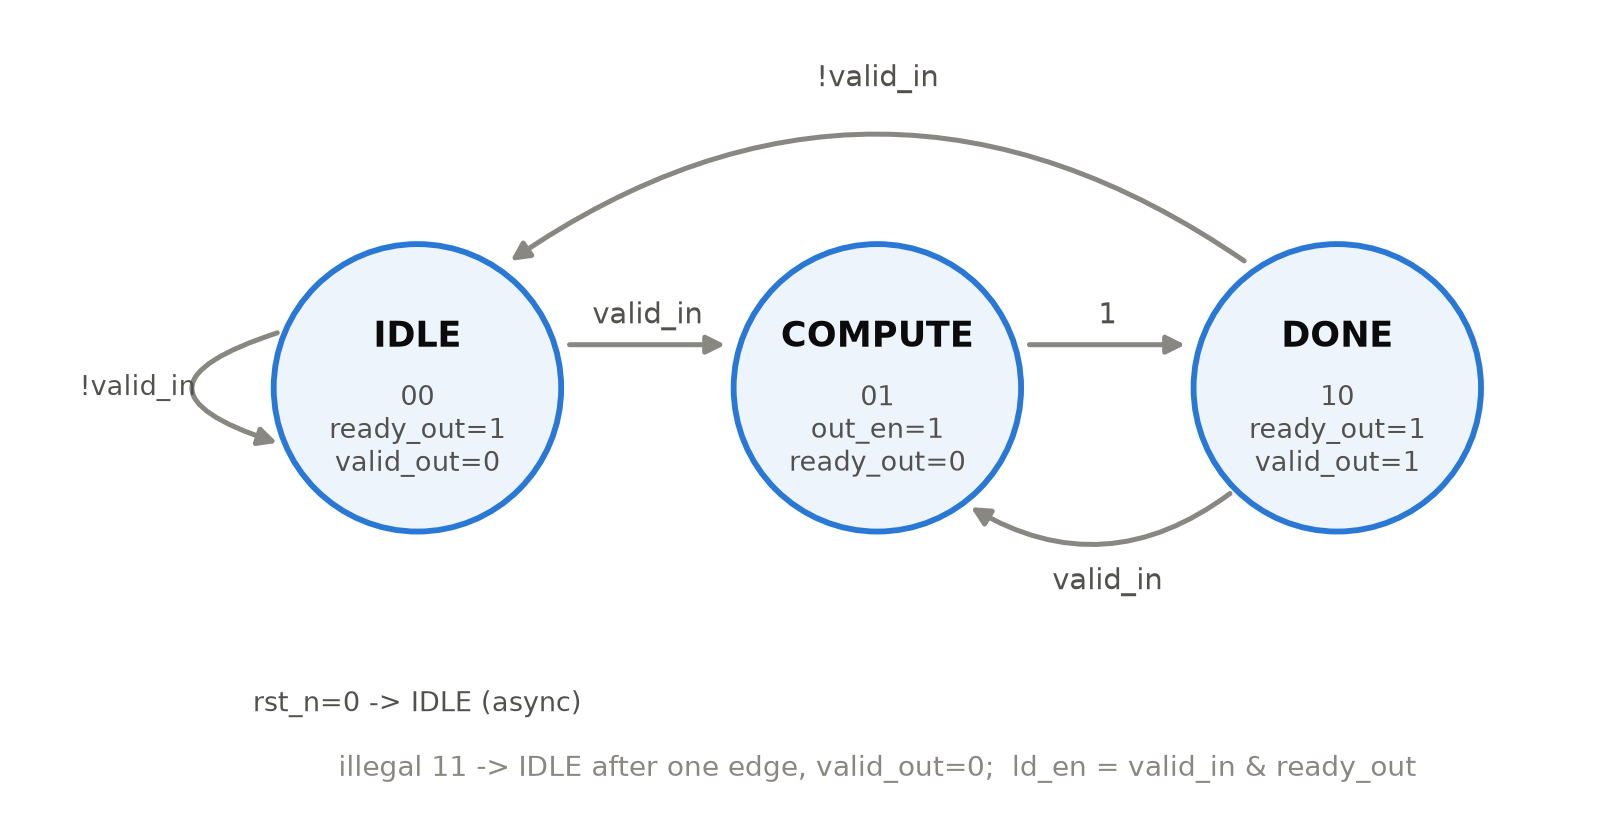
\includegraphics[width=0.92\columnwidth]{fsm.png}
\caption{Moore controller: state codes, outputs and transitions.}
\label{fig:fsm}
\end{figure}

\section{Verification}
A self-checking SystemVerilog testbench runs on Verilator and compares every output against vectors
from an independent Python golden model. Table~\ref{tab:ver} lists the cases. Fig.~\ref{fig:wave}
shows back-to-back transfers: an input accepted at clock edge $k$ produces \texttt{valid\_out} at
edge $k+2$, and the next result follows two cycles later.

\begin{table}[t]
\centering
\caption{Verification cases (Verilator, self-checking)}
\label{tab:ver}
\begin{tabular}{@{}llc@{}}
\toprule
Case & Scenario & Result \\
\midrule
1 & directed vectors after reset & \metric{sim.case1.status} \\
2 & back-to-back, latency and throughput & \metric{sim.case2.status} \\
3 & random \texttt{valid\_in} bubbles (30\%) & \metric{sim.case3.status} \\
4 & async reset in COMPUTE and in DONE & \metric{sim.case4.status} \\
5 & exhaustive, \metric{sim.exhaustive.checked} vectors, \metric{sim.exhaustive.errors} errors & \metric{sim.case5.status} \\
-- & illegal state \texttt{2'b11} & \metric{sim.case_illegal.status} \\
\bottomrule
\end{tabular}
\end{table}

\begin{figure}[t]
\centering
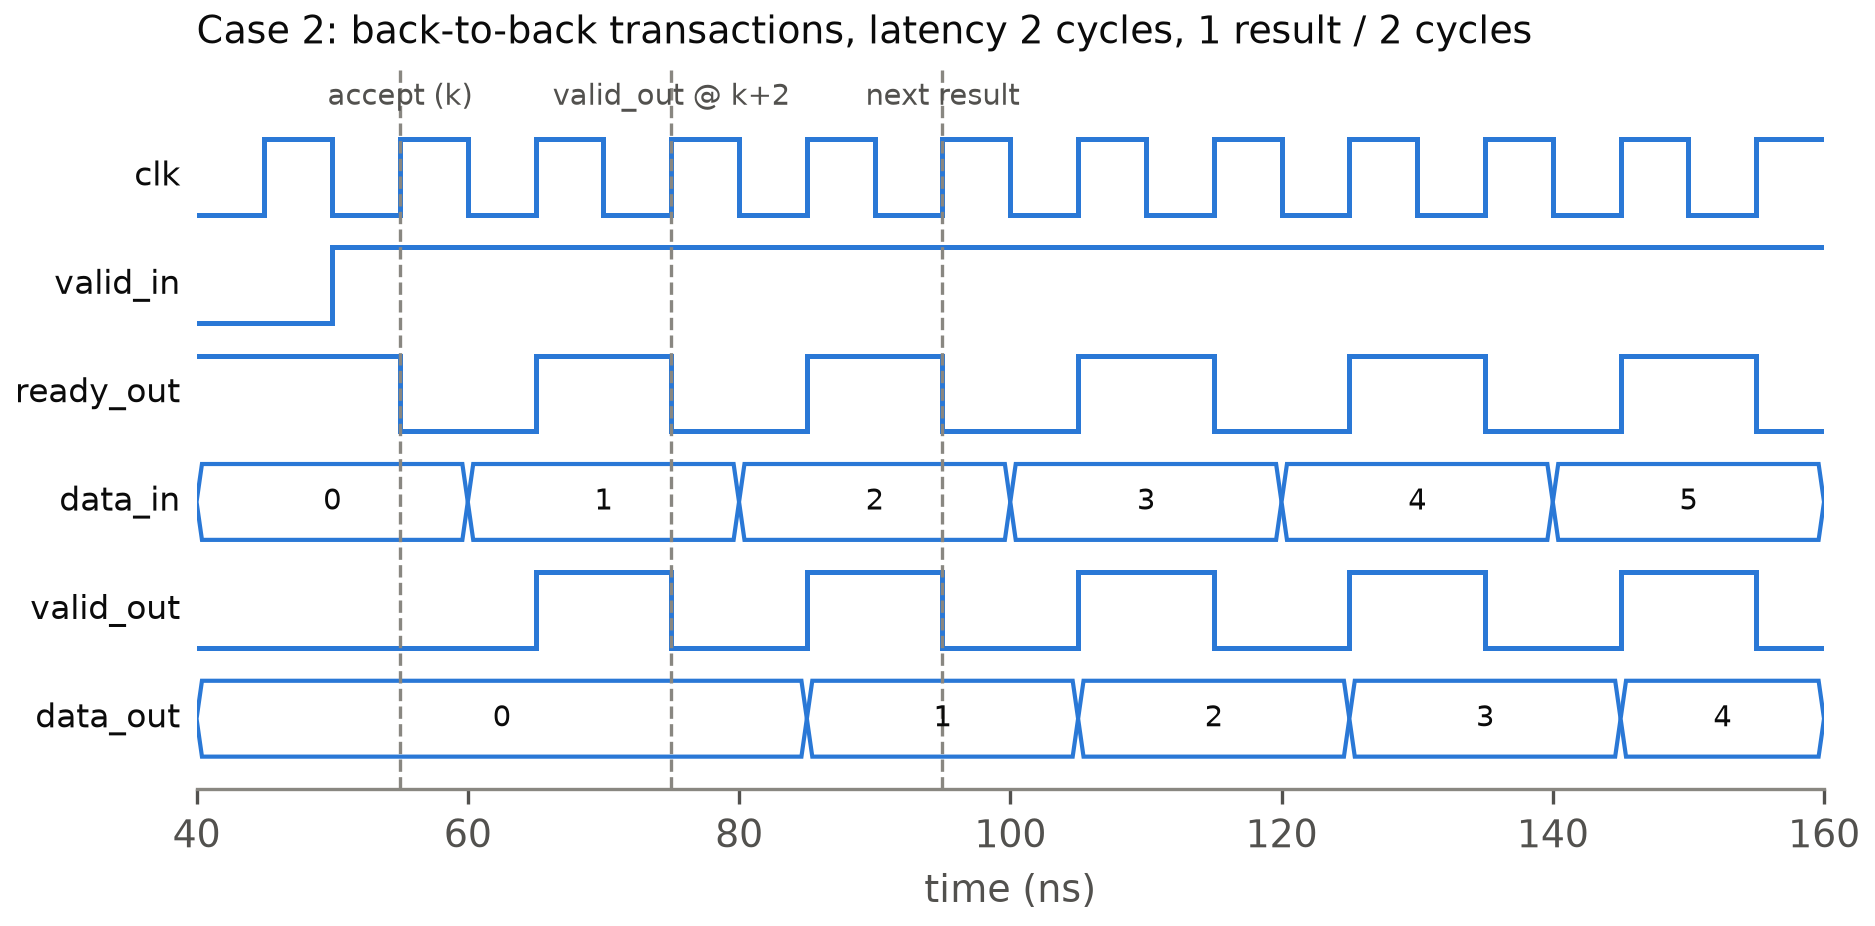
\includegraphics[width=\columnwidth]{wave_case2.png}
\caption{Case 2 waveform: latency of two cycles, one result every two cycles.}
\label{fig:wave}
\end{figure}

\section{Synthesis and Physical Design}
Yosys maps the design to \texttt{sky130\_fd\_sc\_hd} cells: \metric{synth.top.cell_count} cells,
\metric{synth.top.area_um2}\umsq, i.e.\ \metric{synth.top.nand2_eq} NAND2 equivalents against a
budget of 500. With a 10\,ns clock and 2\,ns input/output delays, OpenSTA reports a worst setup slack
of \metric{sta.synth.wns_setup_ns}\,ns at the typical corner; the register-to-register critical path
\texttt{\metric{sta.synth.crit_path}} arrives after \metric{sta.synth.crit_arrival_ns}\,ns.

Fig.~\ref{fig:ad} compares the CSLA with a 4-bit RCA. With hierarchy kept, the CSLA is faster
(\metric{cmp.csla4.delay_ns} vs.\ \metric{cmp.rca4.delay_ns}\,ns) but larger
(\metric{cmp.csla4.area_um2} vs.\ \metric{cmp.rca4.area_um2}\umsq), so its area--delay product is
worse. When ABC may flatten the logic, both shrink and slow down; the flat CSLA keeps the lower delay
(\metric{cmp.csla4_flat.delay_ns} vs.\ \metric{cmp.rca4_flat.delay_ns}\,ns) and gives the best
area--delay product. At four bits the duplicated upper block costs nearly as much as it saves.

\begin{figure}[t]
\centering
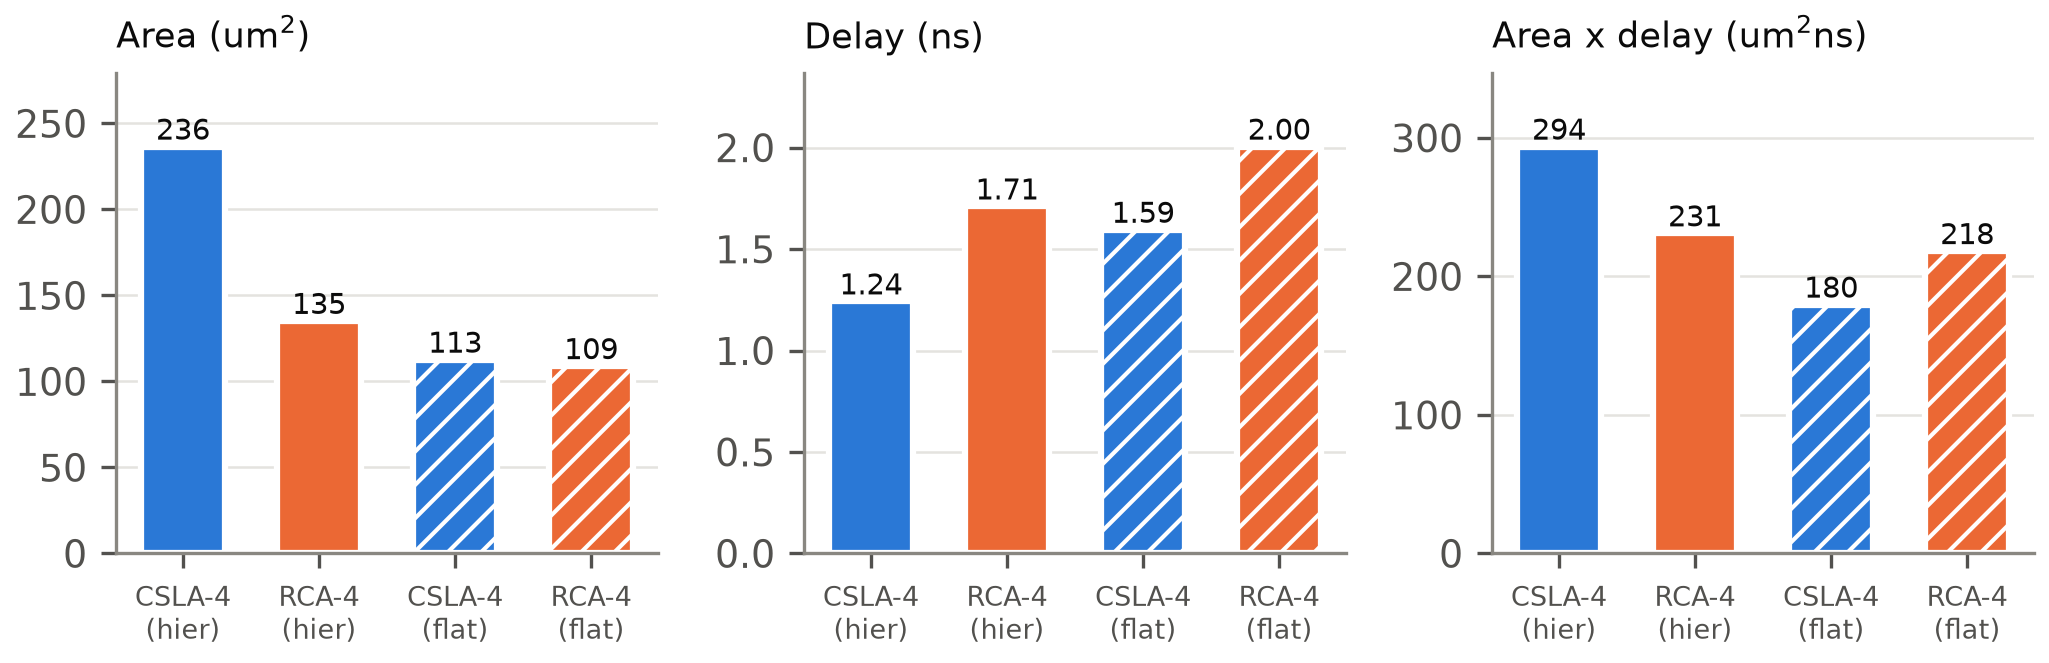
\includegraphics[width=\columnwidth]{area_delay.png}
\caption{CSLA-4 vs.\ RCA-4 after synthesis (typical corner); hatched bars are flattened netlists.}
\label{fig:ad}
\end{figure}

LibreLane places and routes the design with a 55\% core-utilization target and aspect ratio 1
(Fig.~\ref{fig:layout}). Table~\ref{tab:ppa} summarizes signoff. Setup and hold slack are positive in
all nine corners (min/nom/max extraction $\times$ ss/tt/ff), including the recovery/removal checks of
\texttt{rst\_n}. The estimated maximum frequency at the typical corner is
\metric{pnr.fmax_mhz}\,MHz. \metric{pnr5.text_en}

\begin{table}[t]
\centering
\caption{Post-route signoff at 100\,MHz}
\label{tab:ppa}
\begin{tabular}{@{}lr@{}}
\toprule
Metric & Value \\
\midrule
Die area (\textmu m$^2$) & \metric{pnr.die_area_um2} \\
Std cells / final utilization (\%) & \metric{pnr.cell_count} / \metric{pnr.core_util_pct} \\
Setup slack, tt / worst corner (ns) & \metric{pnr.wns_setup_ns} / \metric{pnr.wns_setup_worst_corner_ns} \\
Hold slack, tt / worst corner (ns) & \metric{pnr.wns_hold_ns} / \metric{pnr.wns_hold_worst_corner_ns} \\
$f_{max}$ estimate, tt (MHz) & \metric{pnr.fmax_mhz} \\
DRC Magic / KLayout, LVS errors & \metric{pnr.drc_magic} / \metric{pnr.drc_klayout} / \metric{pnr.lvs_errors} \\
Antenna violations & \metric{pnr.antenna_violations} \\
Total power (mW), wirelength (\textmu m) & \metric{pnr.power_total_mw}, \metric{pnr.wirelength_um} \\
\bottomrule
\end{tabular}
\end{table}

\begin{figure}[t]
\centering
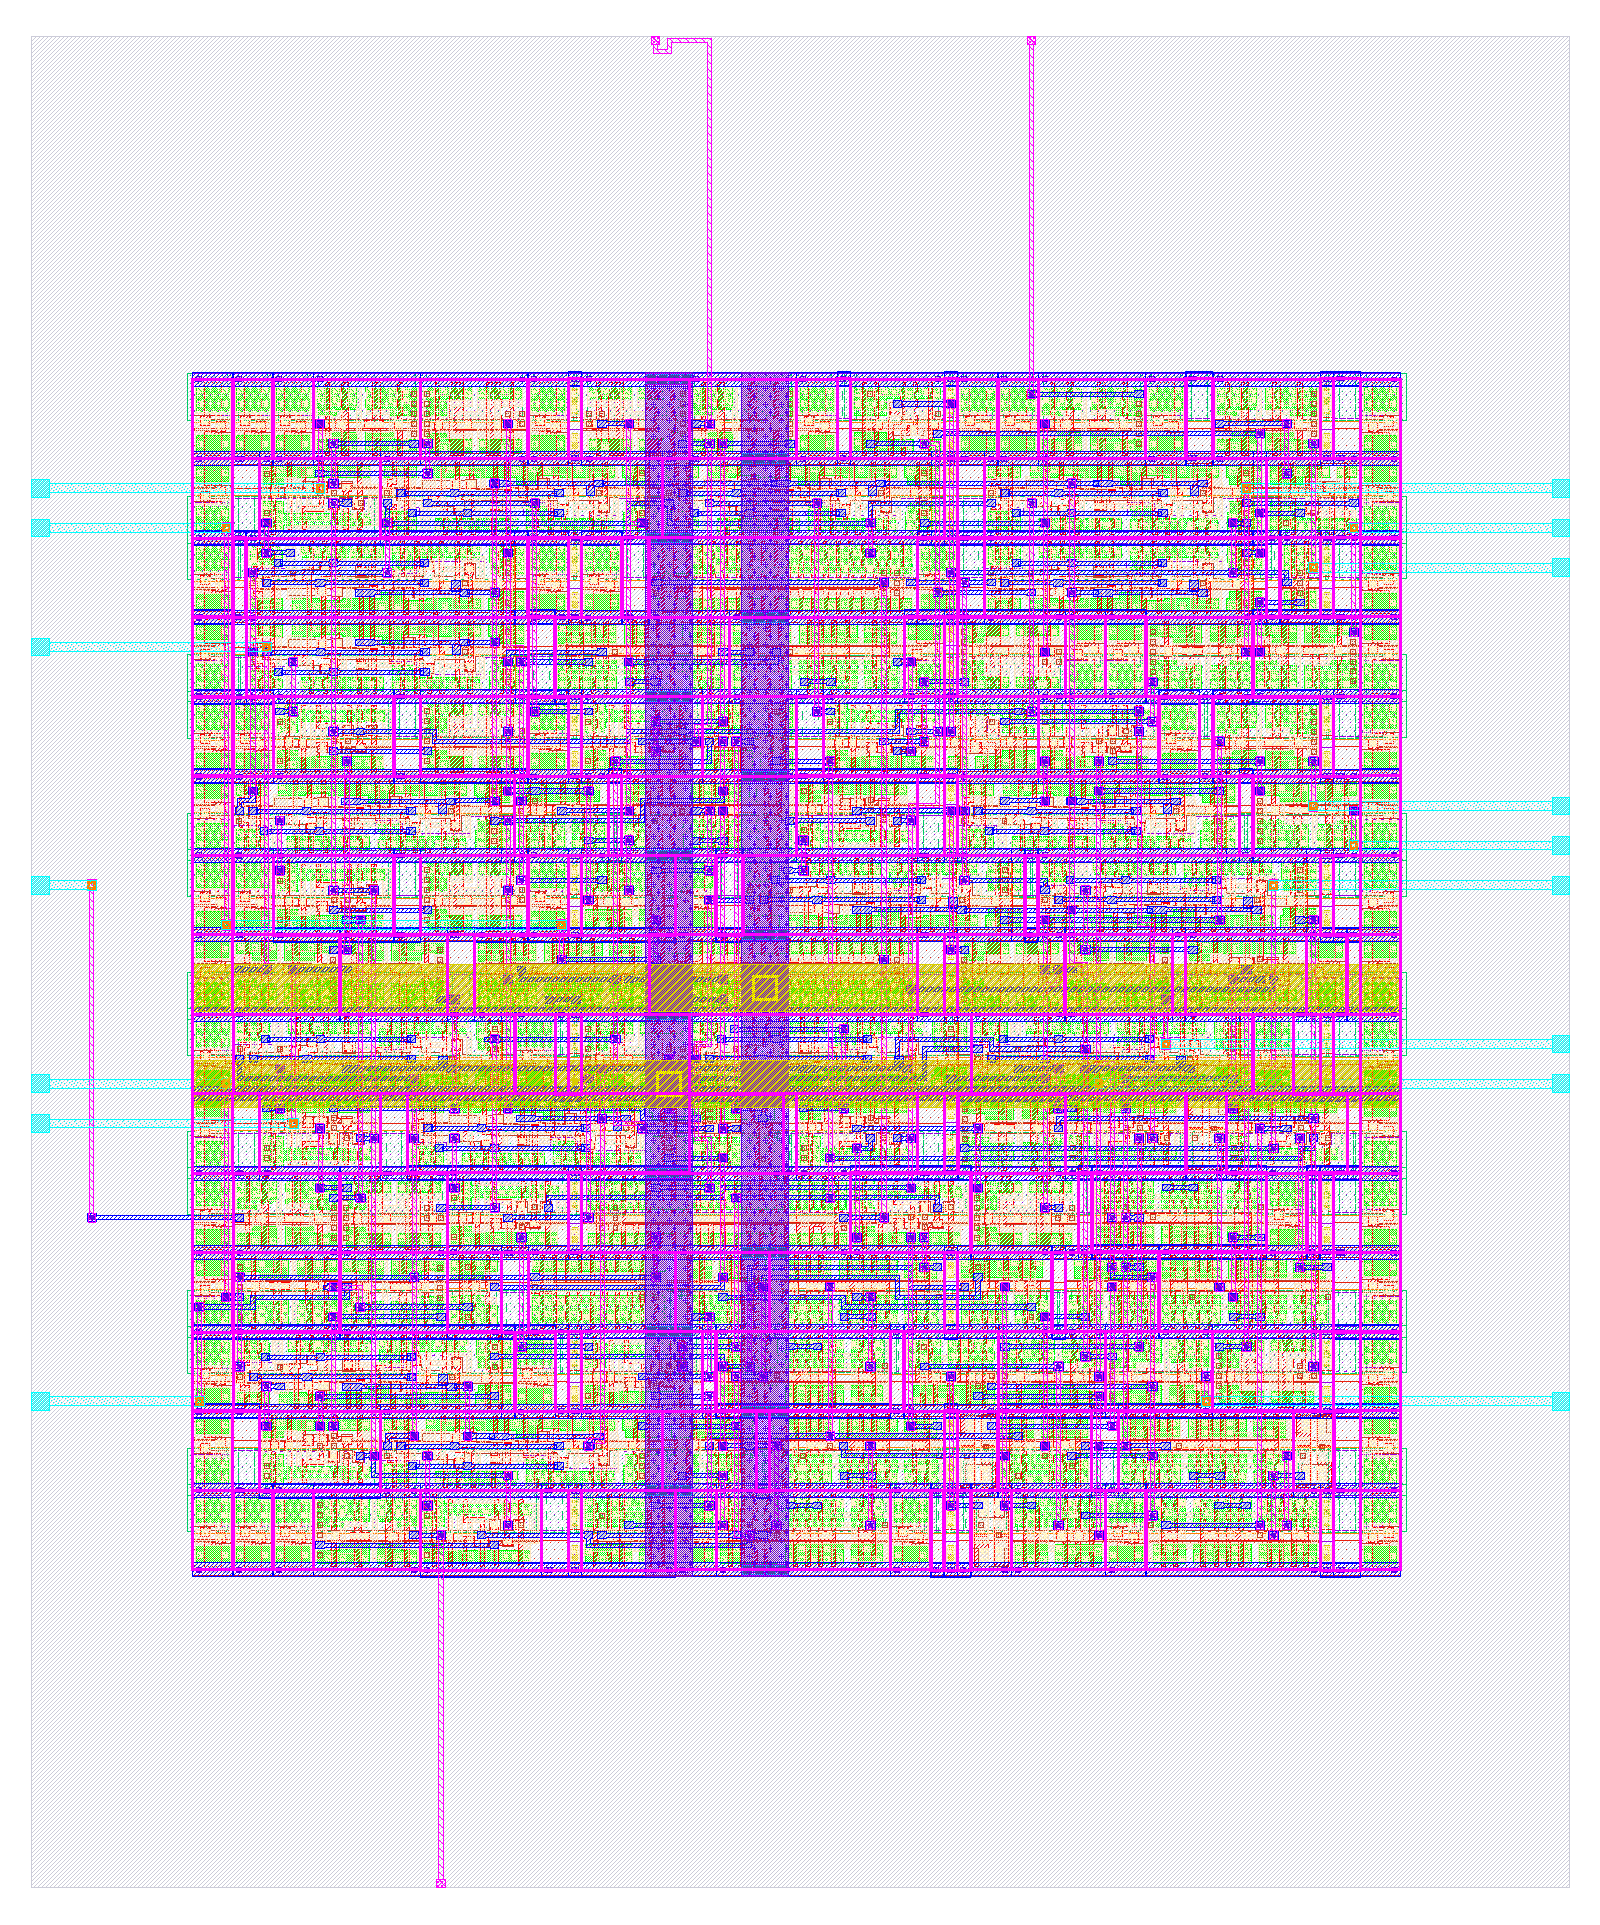
\includegraphics[width=0.62\columnwidth]{layout_top.png}
\caption{Routed layout of \texttt{carryselect4\_top} (LibreLane, SKY130).}
\label{fig:layout}
\end{figure}

\section{Full-Custom Full Adder and Logical Effort}
The leaf cell is a 28-transistor mirror adder: a majority (carry) gate produces $\overline{C_o}$,
a sum gate reuses it to produce $\overline{S}$, and two inverters restore polarity. An FO4 inverter
simulation in ngspice (typical corner) gives $\tau=\metric{le.tau_ps}$\,ps
(FO4 $=\metric{le.fo4_ps}$\,ps) and $p_{inv}=\metric{le.pinv}$ for $W_p/W_n$ =
\metric{le.wp_unit_um}/\metric{le.wn_unit_um}.

We analyse the 2-bit ripple path inside each RCA block, from $a_0$ through two carry gates and two
inverters to $c_2$, which drives three multiplexer select pins
($C_{load}=3\,C_{S,\text{mux2}}$). With $g_{carry}=2$, $g_{inv}=1$ and branching taken from the
transistor widths,
\begin{equation}
F = GBH,\qquad \hat f = F^{1/N},\qquad D = N\hat f + P,
\end{equation}
where $G=\metric{le.G}$, $B=\metric{le.B}$, $H=\metric{le.H}$ and $N=\metric{le.N}$, so
$F=\metric{le.F}$ and $\hat f=\metric{le.fhat}$. With $P = 2p_{carry}+2p_{inv}$ and a simulated
$p_{carry}=\metric{le.p_carry}$, $D=\metric{le.D_est_tau}\,\tau=\metric{le.D_est_ps}$\,ps.
Sizing S1 scales each transistor by its stack depth; sizing S2 also gives the carry-out inverter the
size that Logical Effort assigns to the last stage. S2 is faster in SPICE
(\metric{fa.s2.delay_pre_ps} vs.\ \metric{fa.s1.delay_pre_ps}\,ps) and was laid out.

The layout (Fig.~\ref{fig:fa}) orders the shared polysilicon columns along Euler paths, so the pMOS
and nMOS rows need a single diffusion break. Full-width n- and p-tap rows under the supply rails keep
every device within a few micrometres of a tap, far inside the 15\um\ latch-up limit. The cell
measures \metric{fa.width_um}\,$\times$\,\metric{fa.height_um}\um\ (\metric{fa.area_um2}\umsq),
is DRC-clean with the full SKY130 deck, and matches the schematic in Netgen LVS. Table~\ref{tab:le}
and Fig.~\ref{fig:le} compare the estimate with SPICE. Relative to the schematic simulation the
estimate is off by \metric{le.err_pre_pct}\% (too slow); relative to the extracted netlist it is off
by \metric{le.err_post_pct}\% (too fast). The schematic omits source/drain junction capacitance, and extraction
adds it together with \metric{fa.pex_cap_count} wiring capacitors; Logical Effort folds all of this
into a single parasitic term per stage.

\begin{table}[t]
\centering
\caption{Ripple-carry path delay $a_0\rightarrow c_2$}
\label{tab:le}
\begin{tabular}{@{}lrr@{}}
\toprule
Method & Delay (ps) & LE error \\
\midrule
Logical Effort & \metric{le.D_est_ps} & -- \\
SPICE, schematic & \metric{spice.D_pre_ps} & \metric{le.err_pre_pct}\% \\
SPICE, extracted & \metric{spice.D_post_ps} & \metric{le.err_post_pct}\% \\
\bottomrule
\end{tabular}
\end{table}

\begin{figure}[t]
\centering
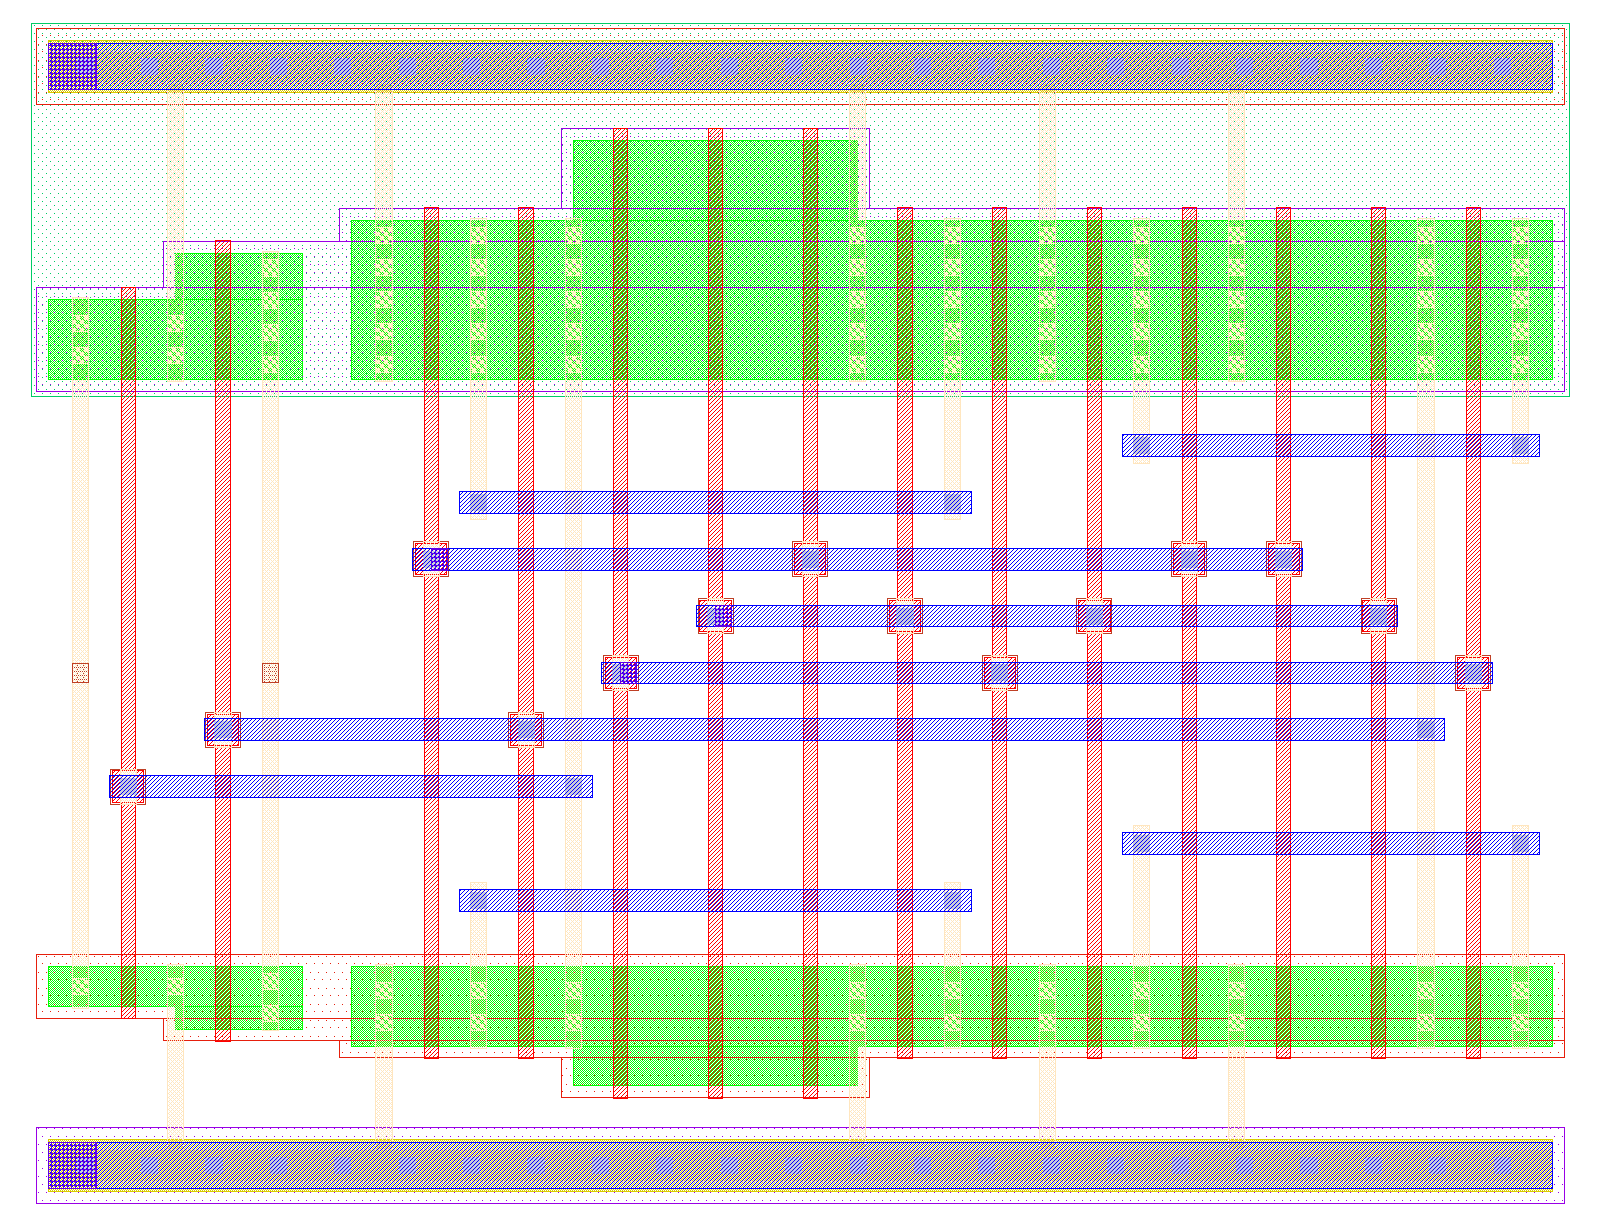
\includegraphics[width=\columnwidth]{fa_layout.png}
\caption{Full-custom 28T mirror full adder in Magic (DRC and LVS clean).}
\label{fig:fa}
\end{figure}

\begin{figure}[t]
\centering
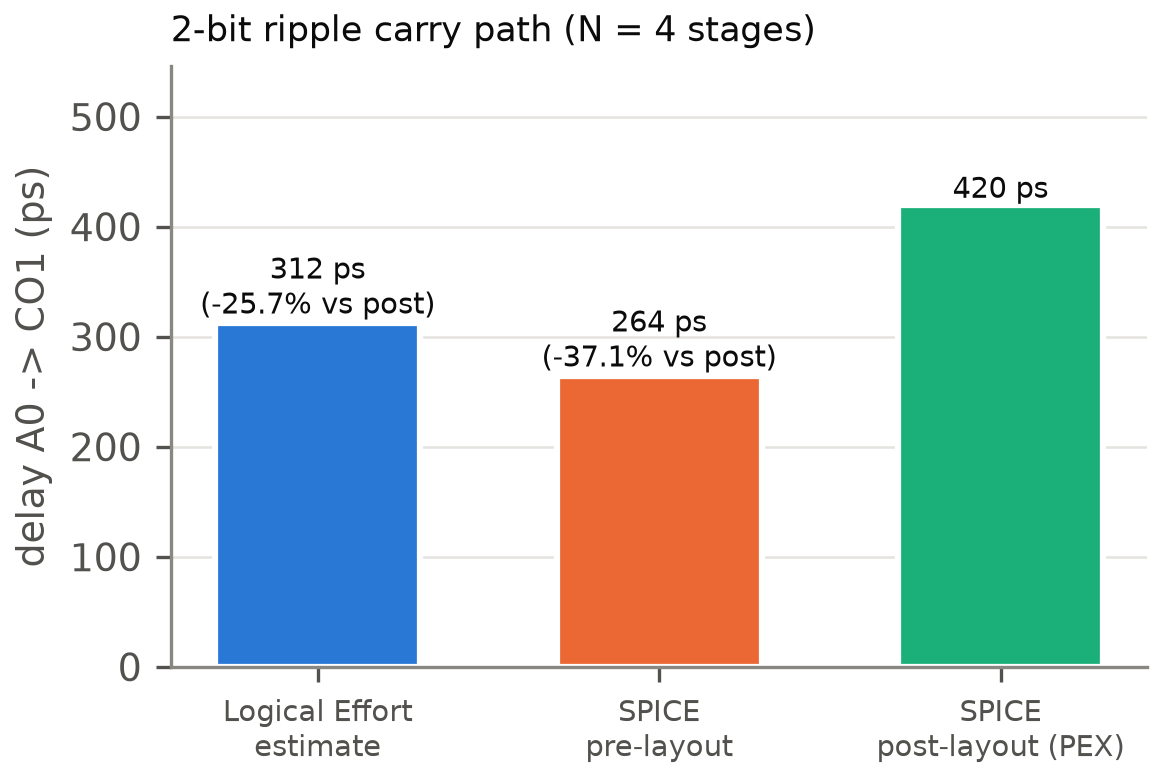
\includegraphics[width=0.85\columnwidth]{le_vs_spice.png}
\caption{Logical Effort estimate vs.\ SPICE before and after extraction.}
\label{fig:le}
\end{figure}

\section{Conclusion}
CarrySelect-4 meets its functional and timing targets: exhaustive simulation passes, the routed
design closes at 100\,MHz in every corner with clean DRC, LVS and antenna checks, and it uses less
than half of its area budget. At four bits the carry-select structure is faster than ripple carry
but does not win on area--delay product unless synthesis is allowed to flatten it. The full-custom
study shows that Logical Effort picks the faster sizing and lands within the pre/post-layout band,
but a layout-aware parasitic term is needed for accurate absolute delay. The custom cell is a
study cell and is not used in the standard-cell flow.

\bibliographystyle{IEEEtran}
\bibliography{refs}

\end{document}
